%\documentclass[dvips,red]{beamer}
%\documentclass[red,xcolor=dvipsnames]{beamer}
\documentclass[xcolor=dvipsnames]{beamer}
\usepackage[utf8]{inputenc}
\usepackage{etex}
\usepackage[T1]{fontenc}
\usepackage[english,german]{babel}
\usepackage{amsmath,amsfonts,amssymb}
%\usepackage{dsfont}
\usepackage{hyperref}
%\usepackage{colortbl}
%\usepackage{rotating}
\usepackage{textcomp}
\usepackage{amsbsy}
\usepackage{marvosym} % Blitz
\usepackage{multicol}
\usepackage{helvet}
\usepackage{xcolor}
\usepackage{graphicx}
\usepackage{braket}
\usepackage{units}
\usepackage{multirow}
%\usepackage{overcite}
%\usepackage{bibgerm}
%\usepackage{inlinebib}
%\usepackage[absolute,overlay]{textpos}
\usepackage{booktabs}
\usepackage{appendixnumberbeamer}
\usepackage{animate}

\usepackage{tikz,pgfplots}
\usetikzlibrary{positioning,fadings,patterns,decorations}

   \tikzfading[name=fade inside,
            inner color=transparent!90,
            outer color=transparent!40]
   \tikzfading[name=fade out,
            inner color=transparent!0,
            outer color=transparent!90]

\pgfdeclaredecoration{stars}{initial}{\state{initial}[width=6pt,next state=star1]
{}
\state{star1}[width=4pt,next state=gap]{\pgfuseplotmark{star}}
\state{gap}[width=4pt,next state=star1]{}
\state{final}{\pgfpathmoveto{\pgfpointdecoratedpathlast}}
}

\pgfdeclaredecoration{starstars}{initial}{\state{initial}[width=6pt,next state=star1]
{}
\state{star1}[width=4pt,next state=star2]{\pgfuseplotmark{star}}
\state{star2}[width=4pt,next state=gap]{\pgfuseplotmark{star}}
\state{gap}[width=4pt,next state=star1]{}
\state{final}{\pgfpathmoveto{\pgfpointdecoratedpathlast}}
}
\tikzset{
dashStar/.style={dash pattern=on 4pt off 4pt,postaction={decorate,decoration=stars}},
dashStarStar/.style={dash pattern=on 4pt off 8pt,postaction={decorate,decoration=starstars}},
}

\definecolor{diplom1}{rgb}{0.0 0.4 1.0}
\definecolor{diplom2}{rgb}{0.0 0.0 0.6}
\definecolor{diplom3}{RGB}{153,0,0} %unirot
\definecolor{diplom4}{RGB}{232,215,23} 
\definecolor{diplom5}{RGB}{51,37,60} 
\definecolor{AUbluedark}{RGB}{0,37,70} 
\definecolor{AUbluelight}{RGB}{0,61,115} 

%\definecolor{diplom1}{rgb}{0,0.75,0.75}
%\definecolor{diplom2}{RGB}{153,0,0}

%\newrgbcolor{diplom1}{0.3 0.6 1.0}
%\newrgbcolor{diplom2}{0.8 0.1 0.7}

%\usetheme{CambridgeUS}
%\usetheme{Madrid}
\usetheme{Pittsburgh}
%\usecolortheme{mycrane}
%\usecolortheme{orchid}
%\usecolortheme{dove}
%\setbeamercolor{background canvas}{bg=black}
%\setbeamercolor{normal text}{fg=white,bg=black}
%\setbeamercolor{title}{fg=white,bg=black}
%\setbeamercolor{frametitle}{fg=white,bg=black}
%\usebeamercolor[fg]{normal text}
\usecolortheme[named=AUbluelight]{structure}
%\setbeamercolor*{block body}{bg= white}
%\setbeamercolor*{block title}{bg= diplom2}

%\setbeamercolor{itemize item}{fg=white}
%\setbeamercolor{itemize subitem}{fg=white}
%\setbeamercolor{itemize subsubitem}{fg=white}

\setbeamercovered{transparent}

\beamertemplatenavigationsymbolsempty


%Finde die Bilder
\graphicspath{{bilder/}}

\setcounter{tocdepth}{1}
\newcommand{\nocontentsline}[3]{}
\newcommand{\tocless}[2]{\bgroup\let\addcontentsline=\nocontentsline#1{#2}\egroup}
\DeclareMathOperator\erfc{erfc}

\begin{document}
 

\title[]
{Collaborating using git}
\subtitle{Shared Repositories}
\author[E. Fasshauer]{Elke Fasshauer}
\institute[]{University of Tübingen}
\date[9.11.21]{9th November 2021}

%\titlegraphic{\includegraphics[scale=0.15]{pumuckl_jonglage.pdf}}

% Title page
\begin{frame}
\titlepage
\end{frame}

%\begin{frame}{Where to go for the exercise}

\begin{center}
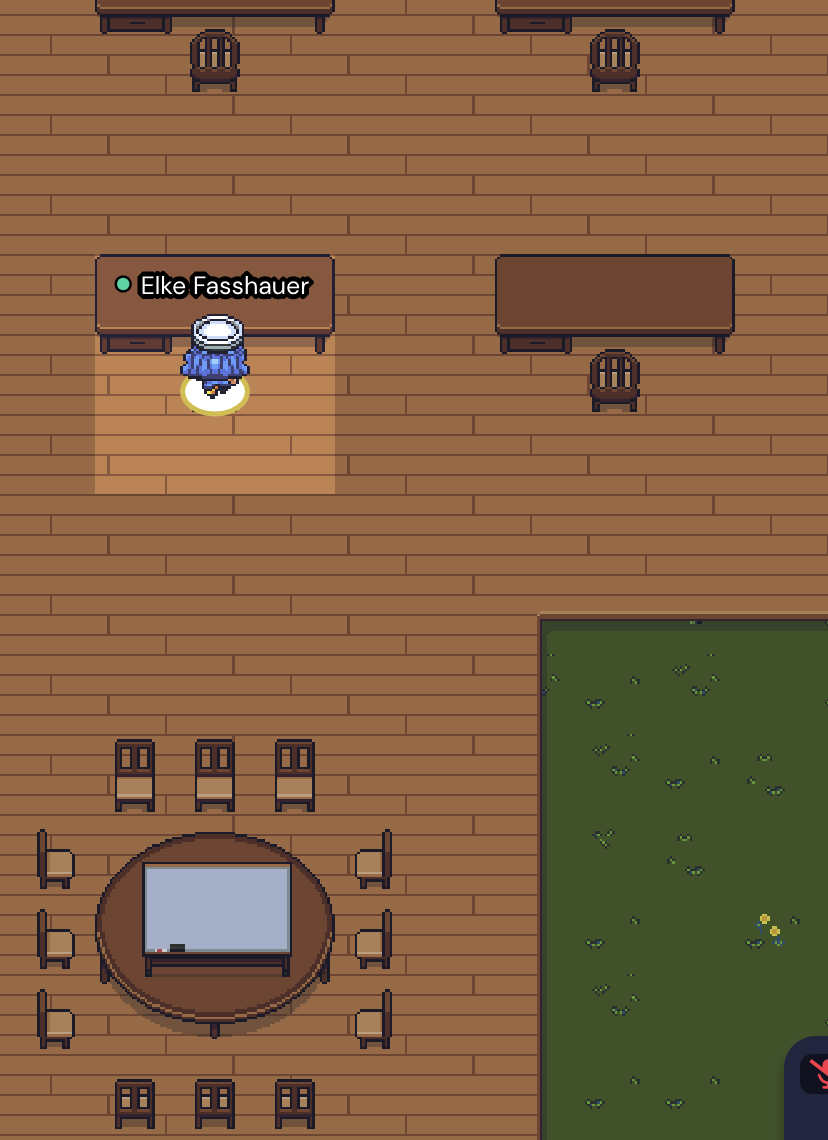
\includegraphics[width=0.45\textwidth]{pics/navigation/sit_small_desk_2.png}
\hfill
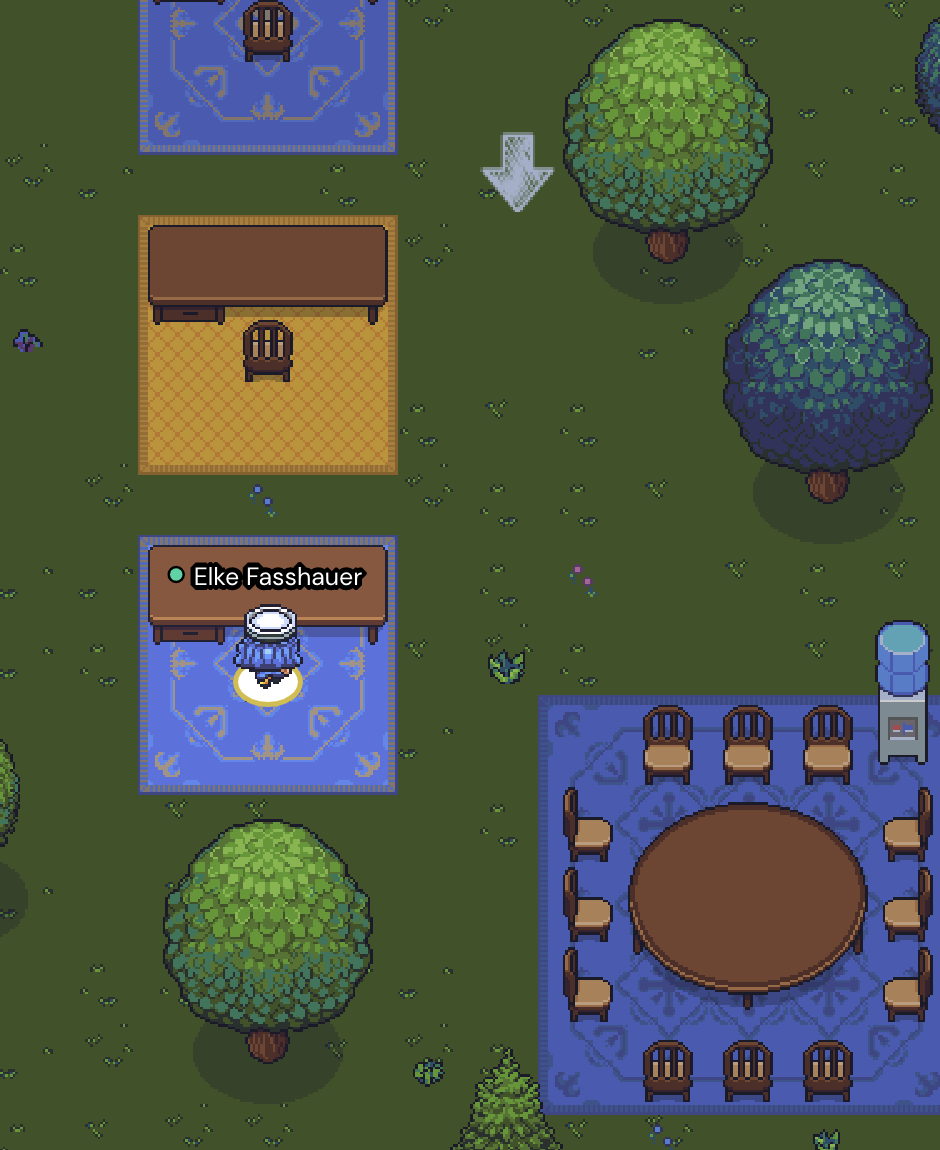
\includegraphics[width=0.45\textwidth]{pics/navigation/sit_small_desk_1.png}
\end{center}

\end{frame}

\begin{frame}{Goal}
\Large

\begin{center}
Write collection of useful commands that a student starting in the
group will need.
\end{center}

%\onslide<2->{
%\begin{block}{}
%\begin{semiverbatim}
%\$ git merge main
%
%\onslide<3->{
%\$ git checkout main
%}
%
%\onslide<4->{
%\$ git merge typo
%}
%
%\onslide<5->{
%\$ git branch -d typo
%}
%
%\onslide<6->{
%\$ git branch
%}
%
%
%
%\only<7->{
%* \textcolor{green}{main}
%
%new\_content
%}
%\end{semiverbatim}
%\end{block}
%}
%
%\onslide<8->{
%\begin{block}{What our file looks like}
%\begin{semiverbatim}
%Test
%
%
%first line
%
%
%\end{semiverbatim}
%\end{block}
%}

\end{frame}

\begin{frame}{Topics and teams}
\footnotesize

\begin{columns}
 \column{0.45\textwidth}
   \begin{block}{Basic terminal}
    \begin{itemize}
      \item Andre
      \item Eirik
    \end{itemize}
   \end{block}

   \begin{block}{vi}
    \begin{itemize}
      \item Esra
      \item Joe
      \item Michael
    \end{itemize}
   \end{block}

   \begin{block}{Working remotely}
    \begin{itemize}
      \item Kyle
      \item Reinhold
    \end{itemize}
   \end{block}

 \column{0.45\textwidth}
   \begin{block}{Finding information and other useful commands}
    \begin{itemize}
      \item Adam
      \item Johannes
    \end{itemize}
   \end{block}

   \begin{block}{Submitting, managing jobs on clusters}
    \begin{itemize}
      \item Andres
      \item Mats
      \item Stefan
    \end{itemize}
   \end{block}
\end{columns}

%\onslide<2->{
%\begin{block}{}
%\begin{semiverbatim}
%\$ git merge main
%
%\onslide<3->{
%\$ git checkout main
%}
%
%\onslide<4->{
%\$ git merge typo
%}
%
%\onslide<5->{
%\$ git branch -d typo
%}
%
%\onslide<6->{
%\$ git branch
%}
%
%
%
%\only<7->{
%* \textcolor{green}{main}
%
%new\_content
%}
%\end{semiverbatim}
%\end{block}
%}
%
%\onslide<8->{
%\begin{block}{What our file looks like}
%\begin{semiverbatim}
%Test
%
%
%first line
%
%
%\end{semiverbatim}
%\end{block}
%}

\end{frame}

\begin{frame}{Collaborate in groups}

\begin{center}
 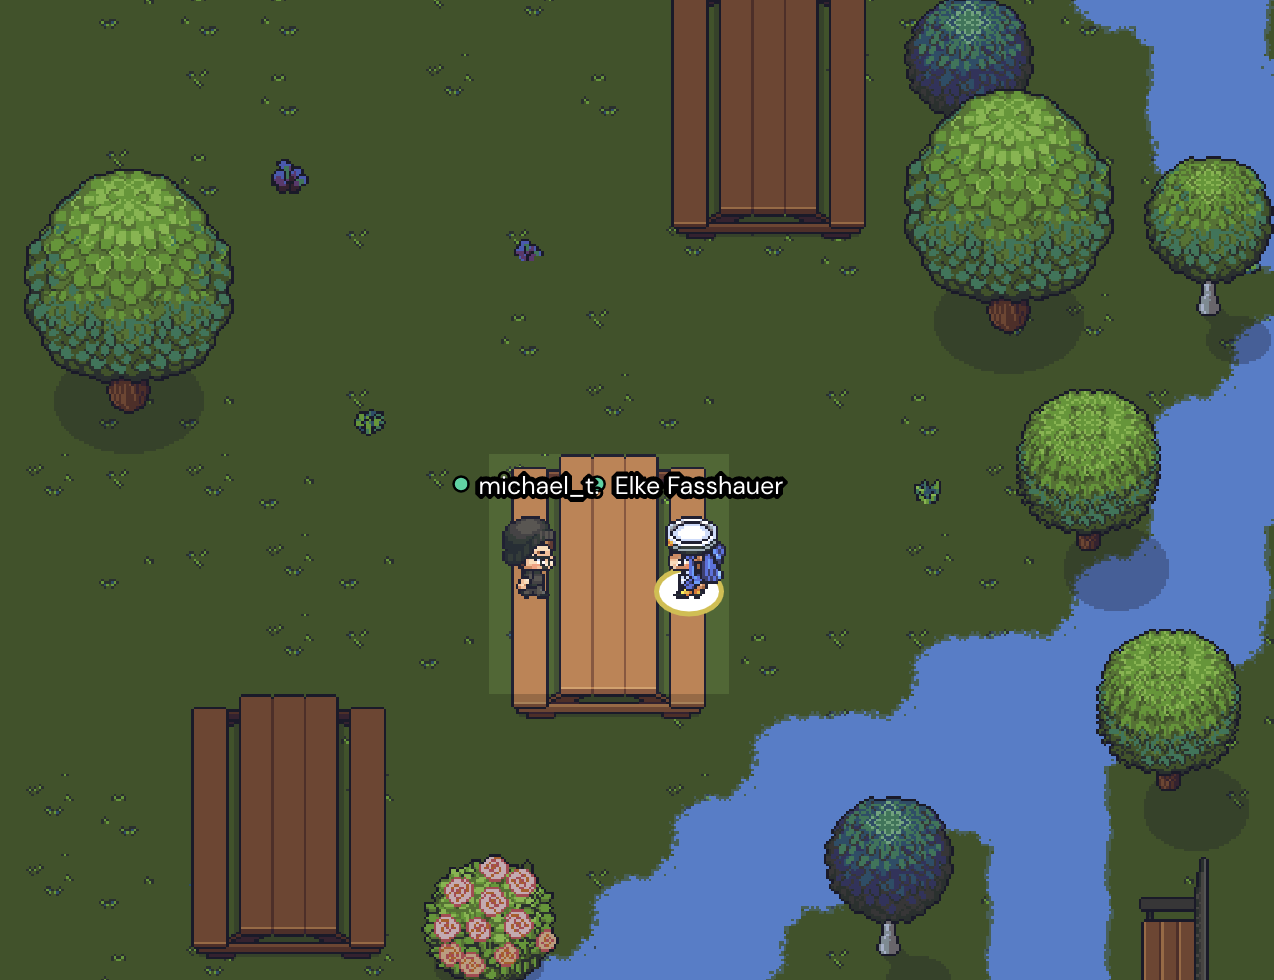
\includegraphics[width=0.8\textwidth]{pics/sit_middle_desk.png}
\end{center}

\end{frame}


\begin{frame}{Motivation}

\begin{center}
  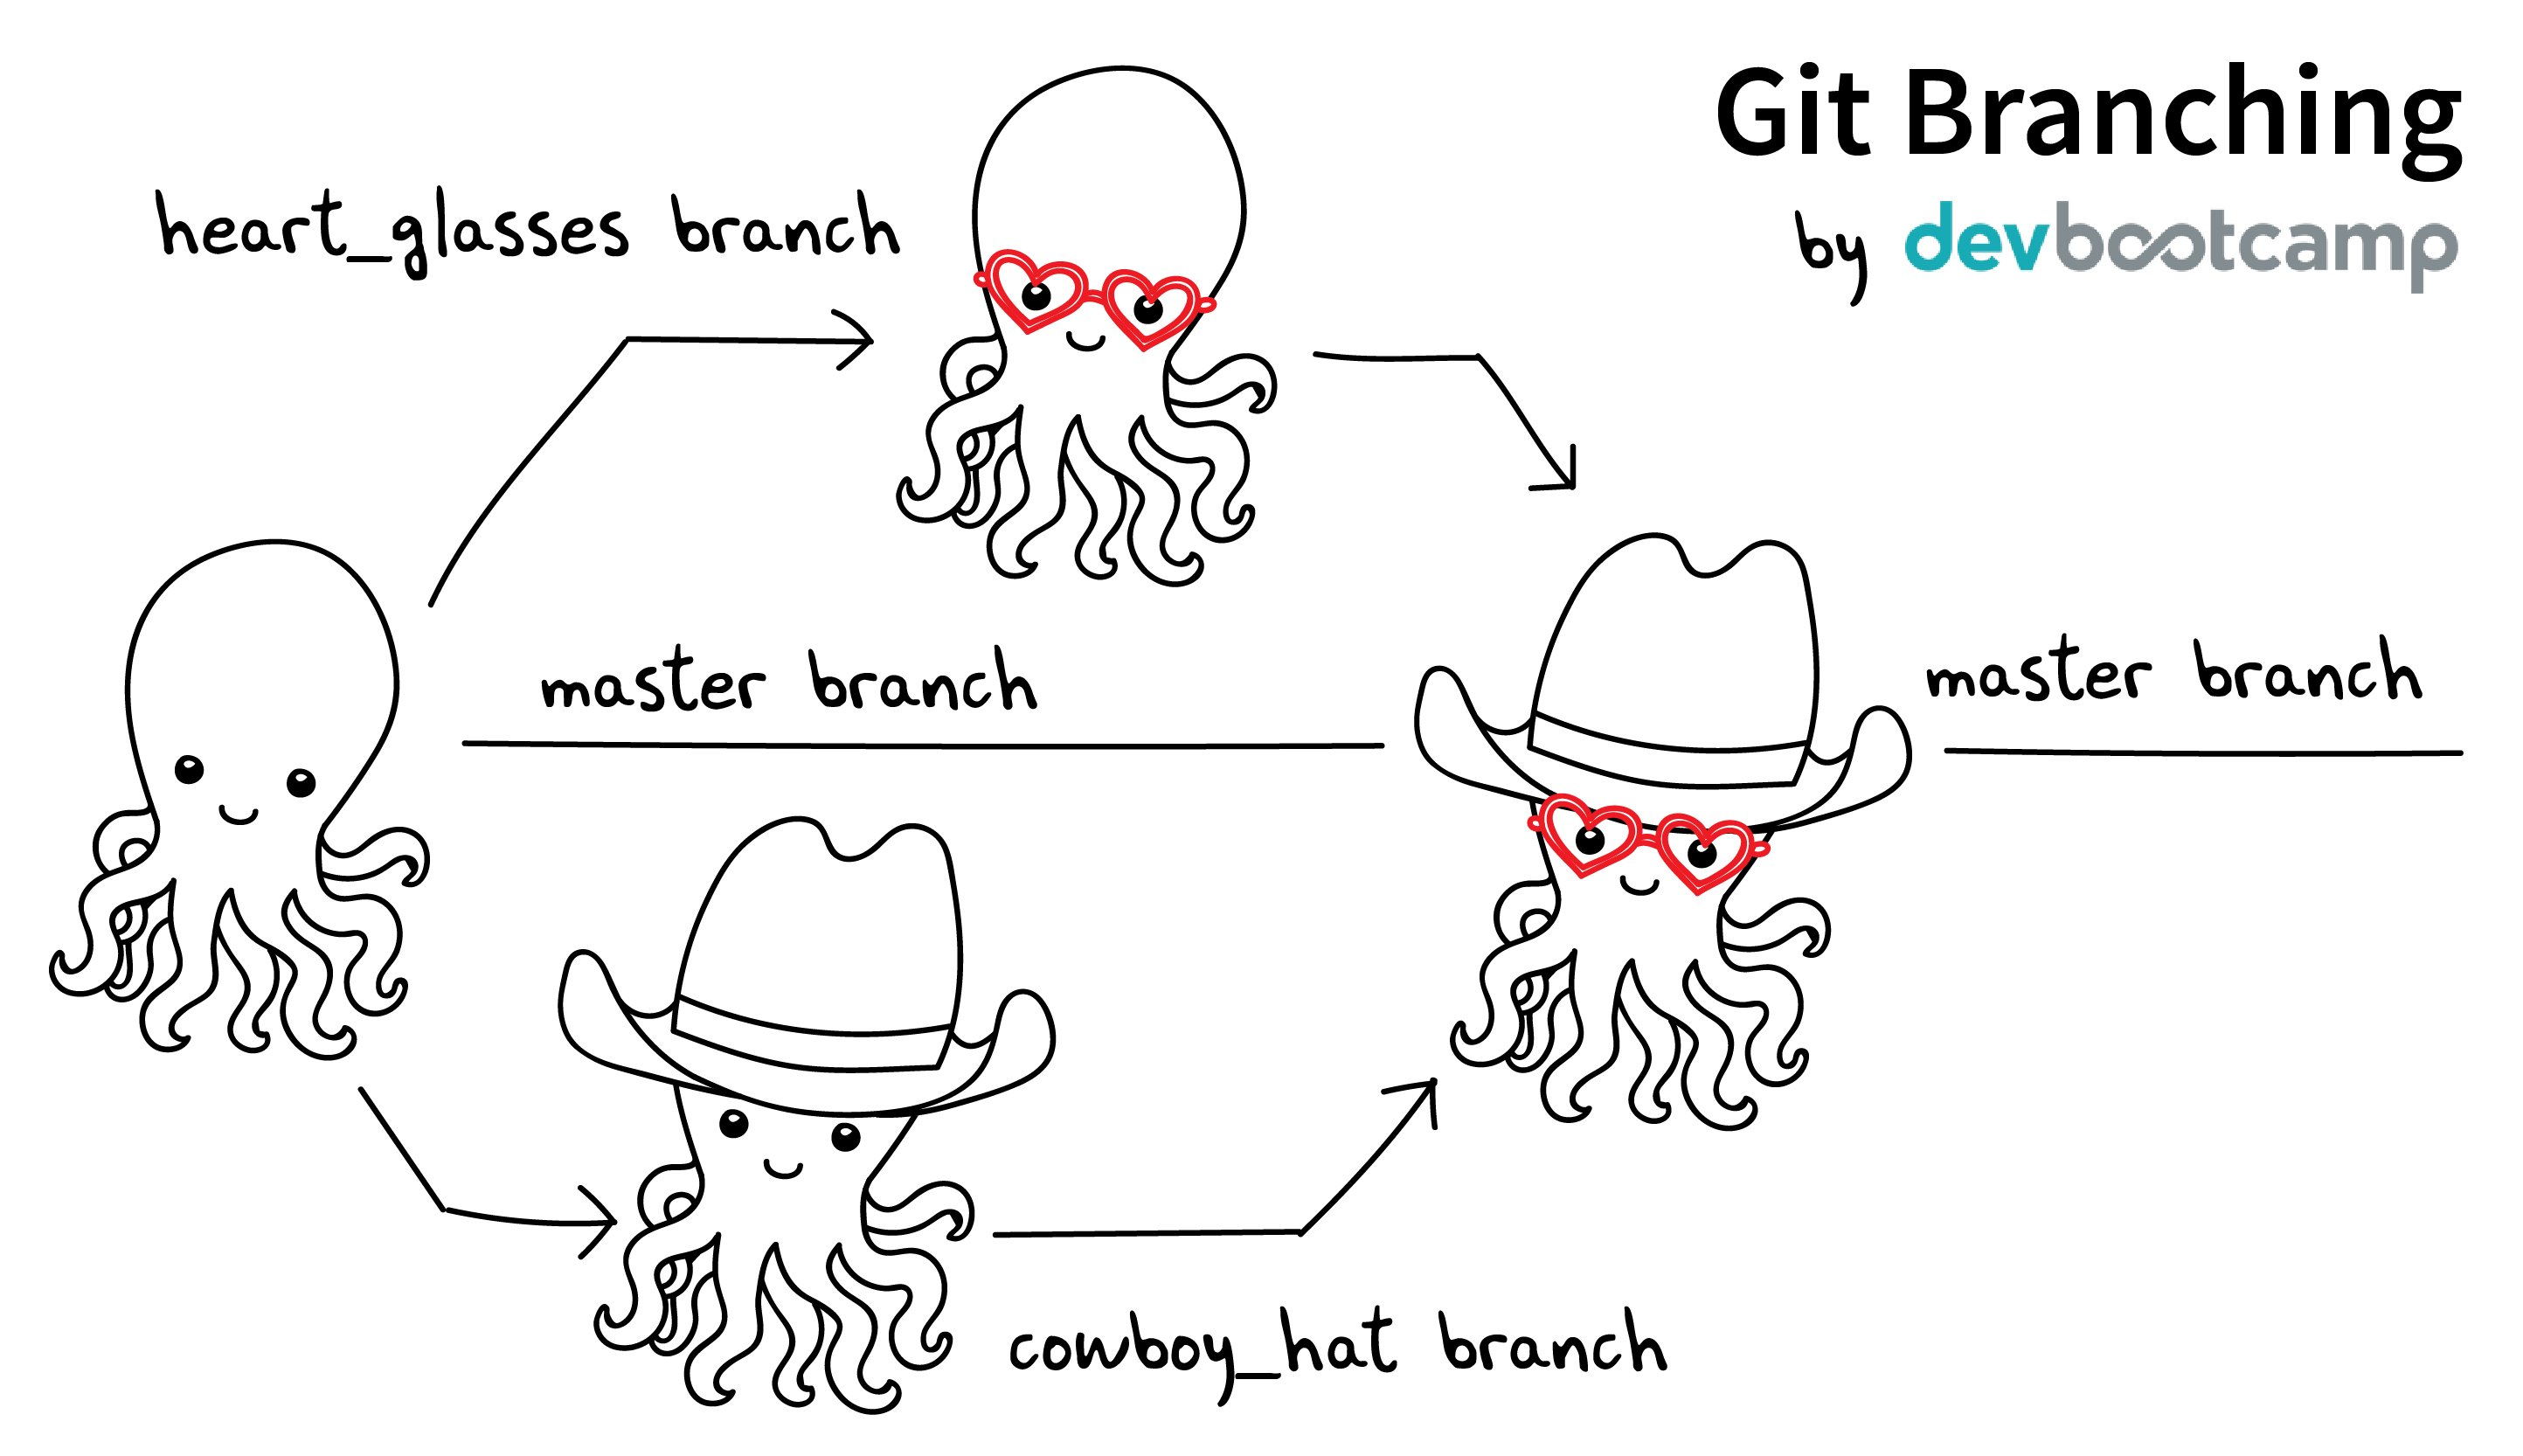
\includegraphics[width=0.8\textwidth]{../01_basics/pics/merging_pic.jpg}
\end{center}


%\begin{semiverbatim}
%git status
%\end{semiverbatim}

\tiny
\begin{tabular}{l}
Coderefinery: \url{https://twitter.com/jay_gee/status/703360688618536960}
\end{tabular}

\end{frame}

\begin{frame}{Platforms}
\footnotesize

\begin{columns}
 \column{0.40\textwidth}
  \only<2-3>{
   
\includegraphics[height=4cm]{pics/Octocat.png}
  }

 \column{0.5\textwidth}
  \only<3>{
   
\includegraphics[height=3cm]{pics/gitlab-logo.png}
  }
\end{columns}

  \only<4>{
   \begin{center}
   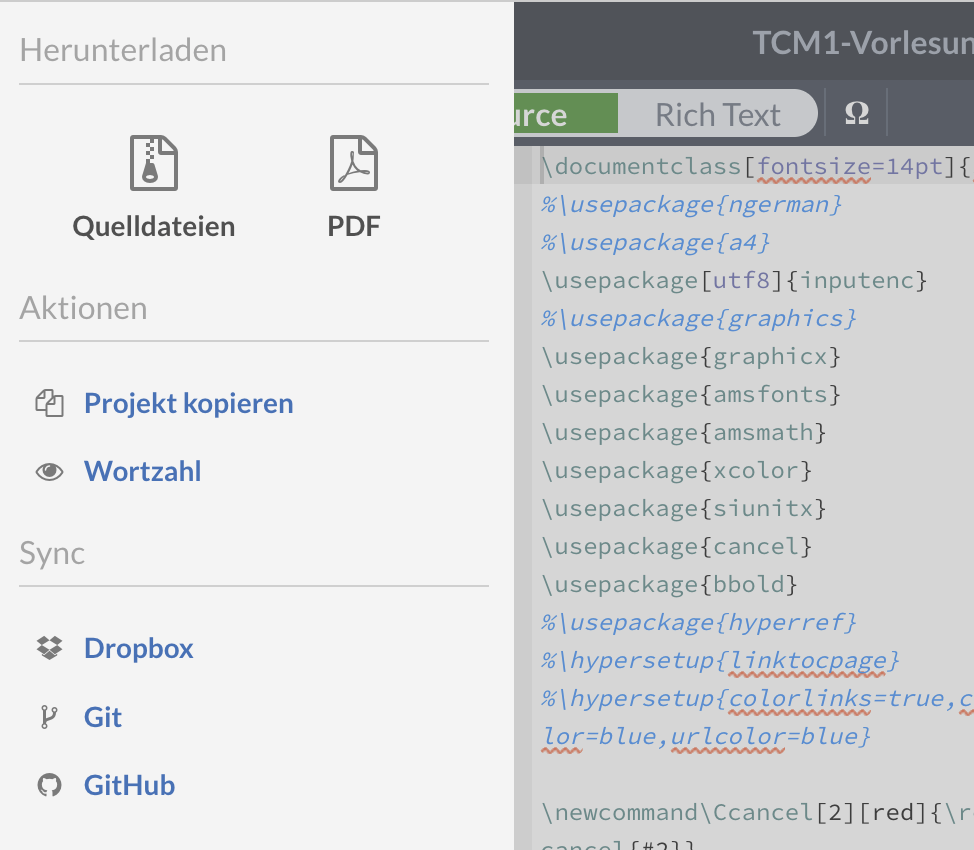
\includegraphics[height=6cm]{pics/git_overleaf.png}
   \end{center}
  }


%\onslide<2->{
%\begin{block}{}
%\begin{semiverbatim}
%\$ git merge main
%
%\onslide<3->{
%\$ git checkout main
%}
%
%\onslide<4->{
%\$ git merge typo
%}
%
%\onslide<5->{
%\$ git branch -d typo
%}
%
%\onslide<6->{
%\$ git branch
%}
%
%
%
%\only<7->{
%* \textcolor{green}{main}
%
%new\_content
%}
%\end{semiverbatim}
%\end{block}
%}
%
%\onslide<8->{
%\begin{block}{What our file looks like}
%\begin{semiverbatim}
%Test
%
%
%first line
%
%
%\end{semiverbatim}
%\end{block}
%}

\end{frame}


\begin{frame}{Central Workflow}

\only<2>{
\begin{center}
 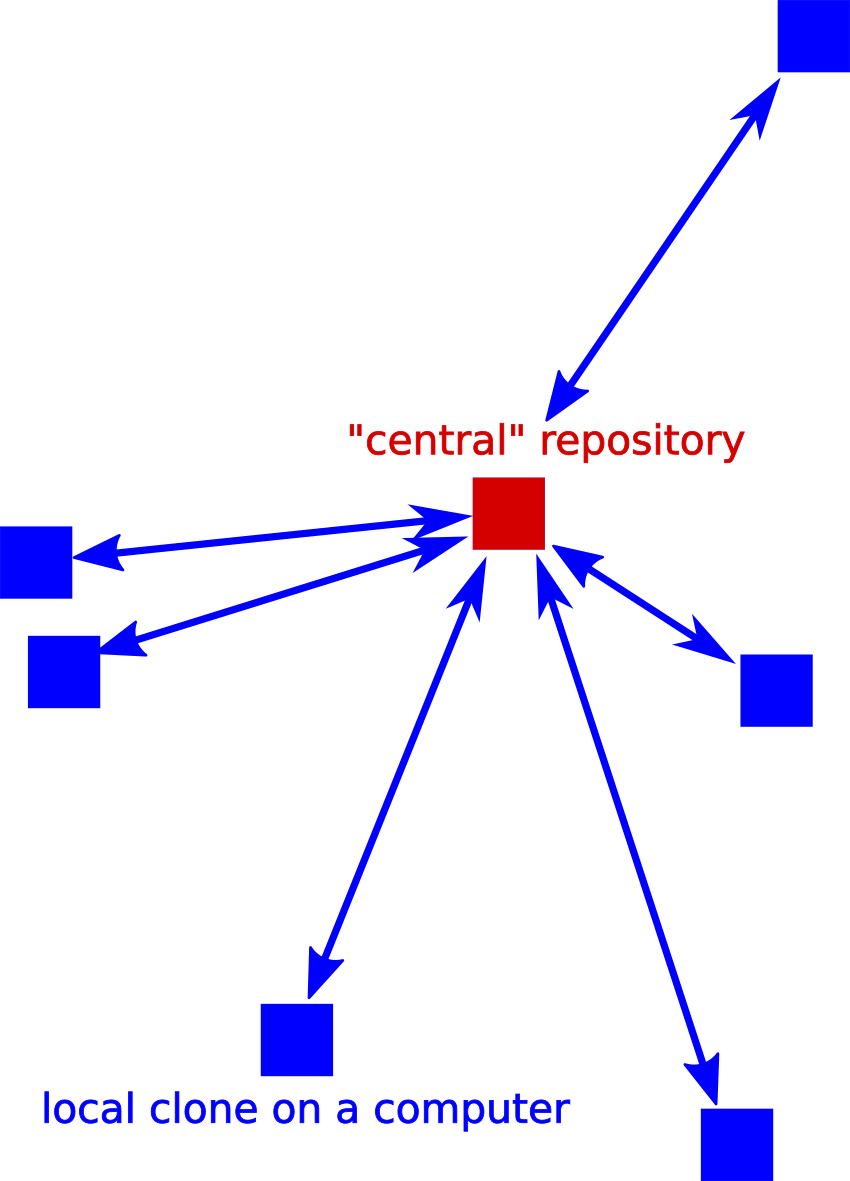
\includegraphics[scale=0.8]{pics/centralized.png}
\end{center}
}

\end{frame}

\begin{frame}{Get the repository}
\footnotesize

\only<2->{
\begin{center}
 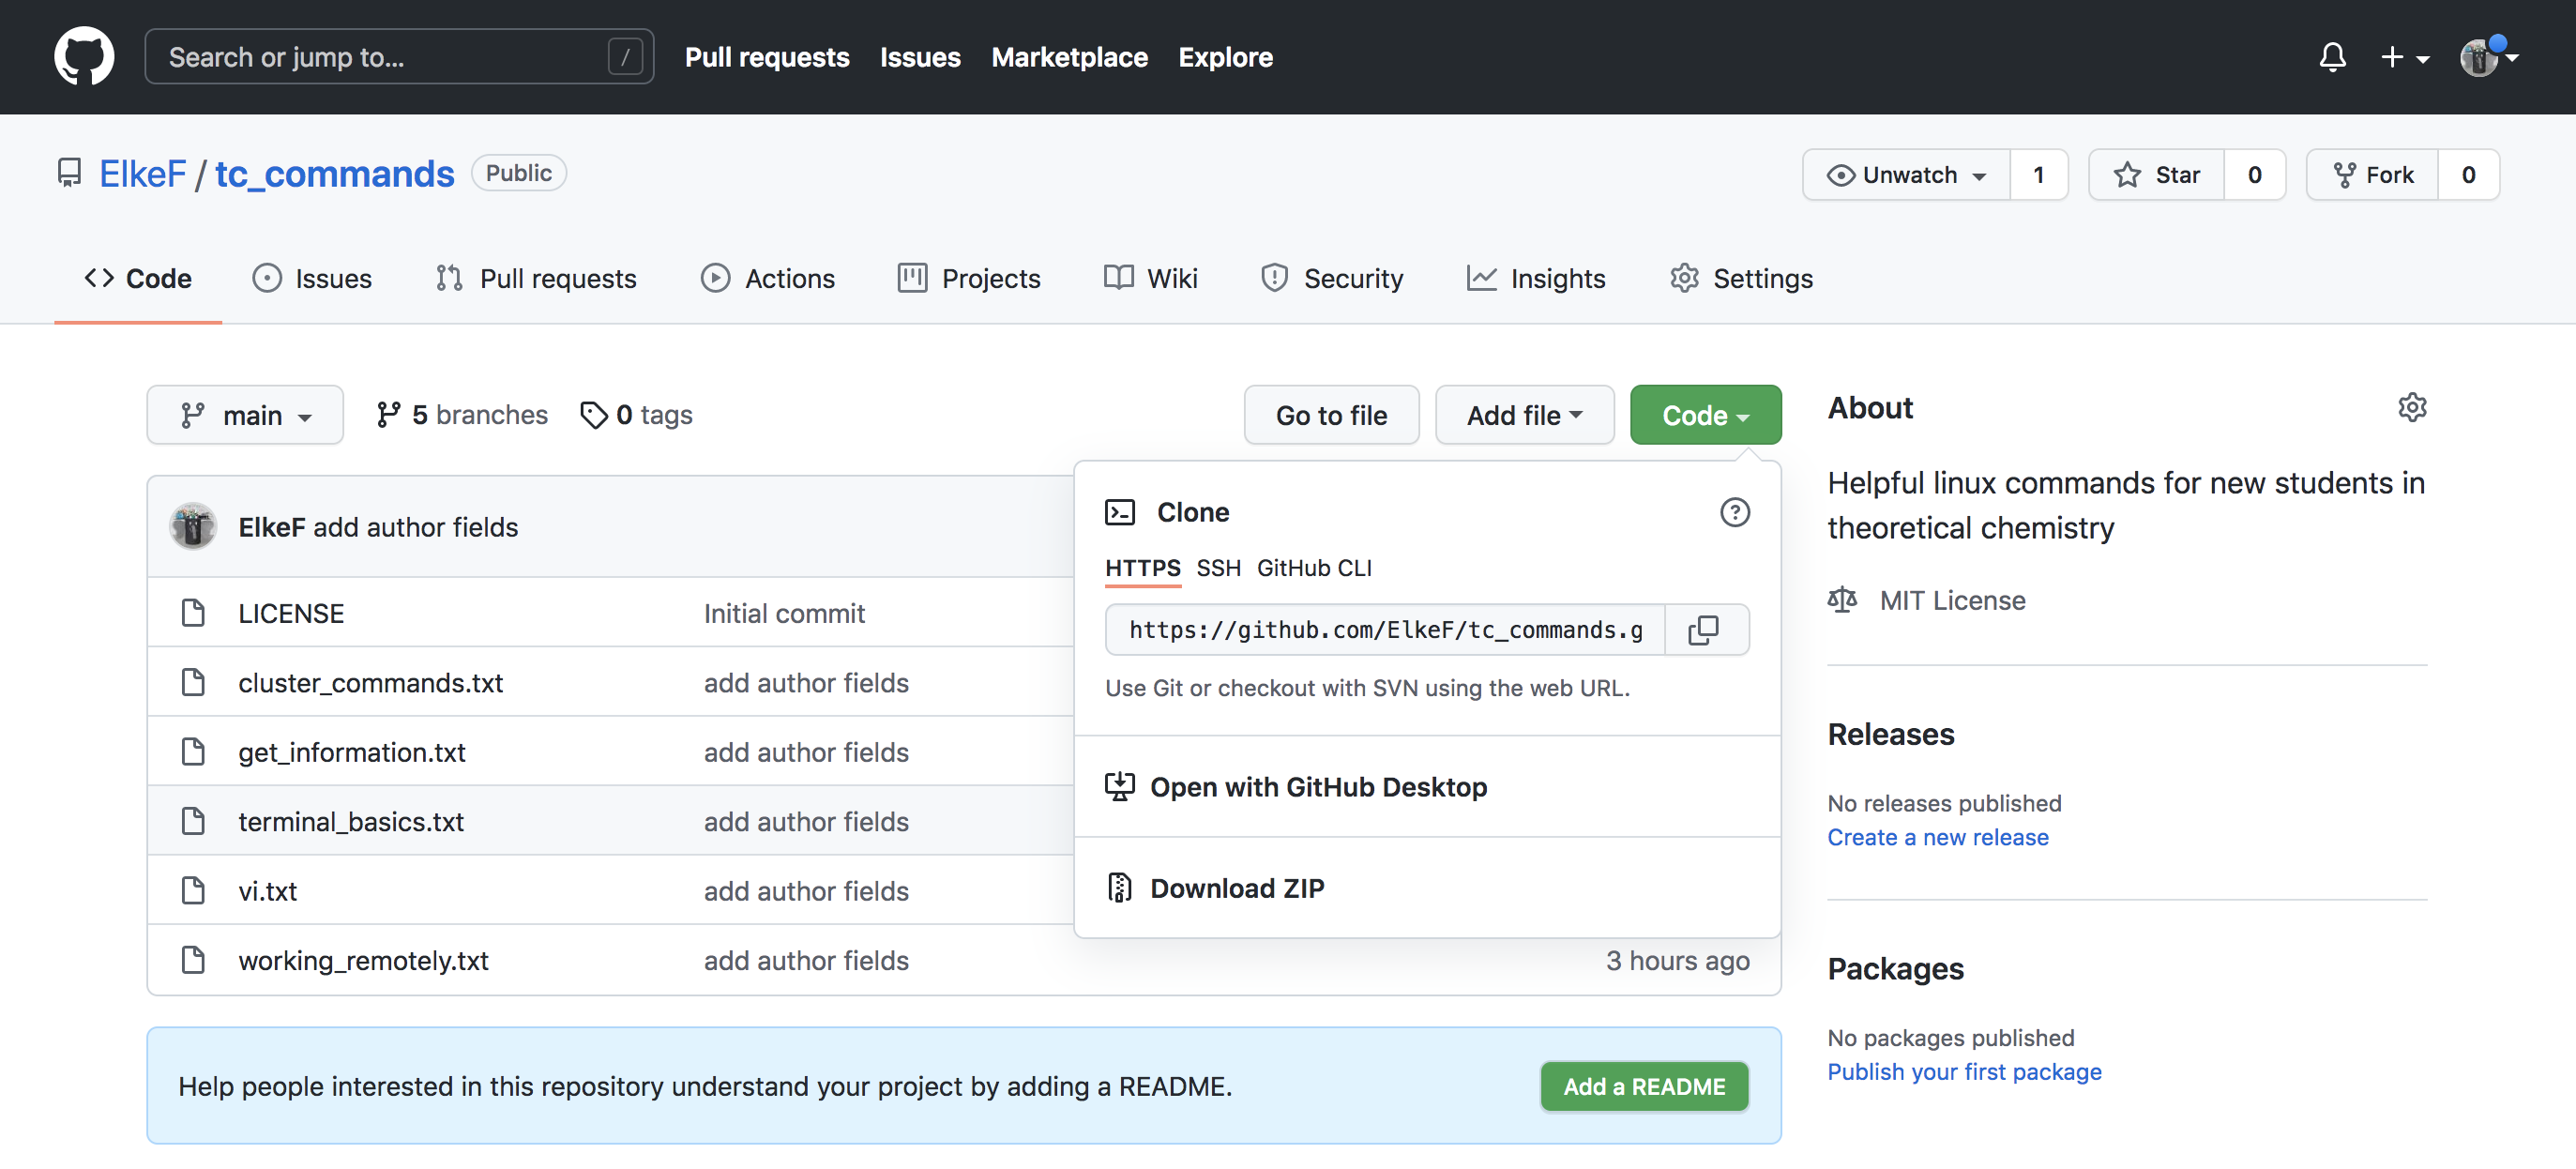
\includegraphics[width=1.0\textwidth]{pics/github_clone}
\end{center}
}

\begin{block}{}
\begin{semiverbatim}

\onslide<3->{
\$ git clone https://github.com/ElkeF/tc\_commands.git TC\_commands
}
\end{semiverbatim}
\end{block}


\end{frame}

\begin{frame}{Remote branches}
\footnotesize

\begin{itemize}
 \item remote branches are not automatically transferred
 \item need to create local branch that tracks remote branch
\end{itemize}


\begin{block}{}
\begin{semiverbatim}

\onslide<2->{
\$ git branch -r
}


\onslide<3->{
  origin/HEAD -> origin/main

  origin/basics

  origin/cluster

  origin/main

  origin/remotely

  origin/vi\_masters
}


\onslide<4->{
\$ git branch basics origin/basics
}
\end{semiverbatim}
\end{block}


\end{frame}

\begin{frame}{Interacting with remote branches: pull, push}
\footnotesize

\begin{block}{Branch off from remote tracking branch}
\begin{semiverbatim}

\onslide<2->{
\$ git checkout basics

\$ git branch feature basics

\$ git checkout feature
}
\end{semiverbatim}
\end{block}

\onslide<3->{
Work, work, work on feature branch
}

\onslide<4->{
\begin{block}{Safely move your changes to collective remote branch}
\begin{semiverbatim}

\$ git checkout basics

\$ git pull

\$ git checkout feature

\$ git merge basics

\$ git checkout basics

\$ git merge feature

\$ git pull

\$ git push
\end{semiverbatim}
\end{block}

}

\end{frame}


\begin{frame}{Conflicts}
\footnotesize

\only<1-2>{
\begin{center}
 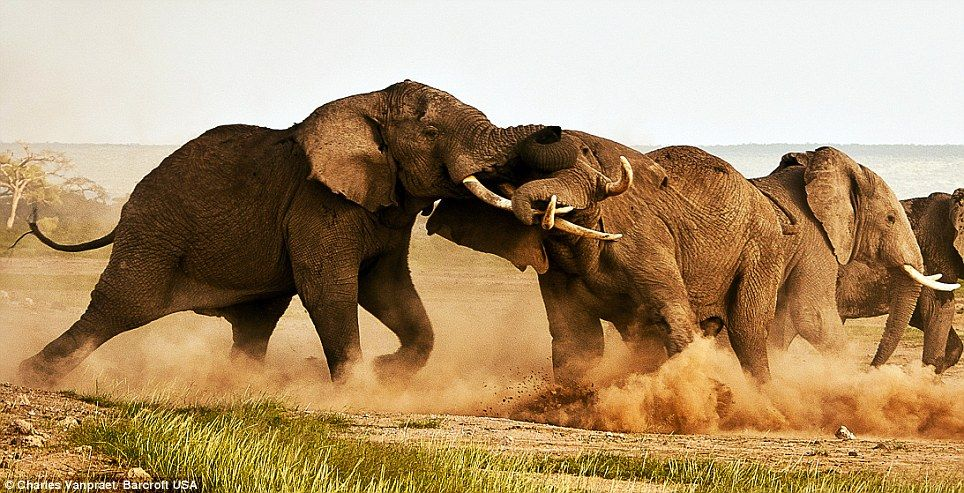
\includegraphics[width=1.0\textwidth]{pics/fight_elephants.jpg}
\end{center}
}

\only<3>{
\begin{center}
 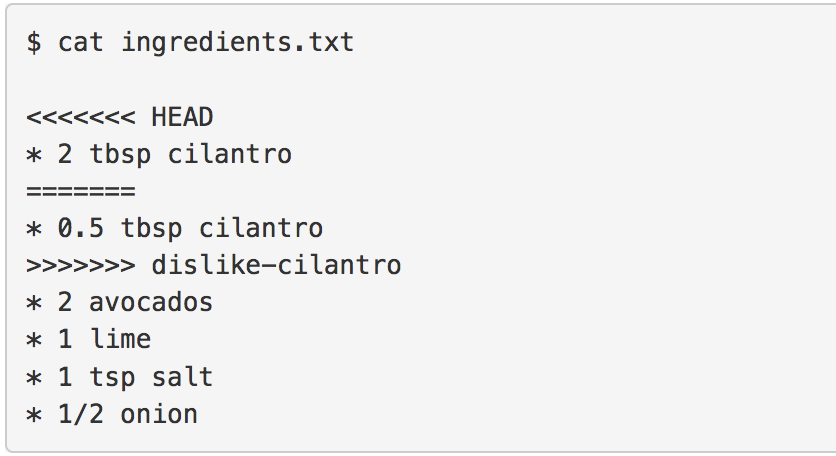
\includegraphics[width=0.7\textwidth]{pics/git_conflict.png}
\end{center}
}

\onslide<2->{
\begin{itemize}
 \item occur when changes are made in the same line of the same document
 \item git does not know, which version to keep and asks you to resolve it
\end{itemize}
}

\end{frame}

\begin{frame}{Conflict Resolution}
\footnotesize

\begin{center}
 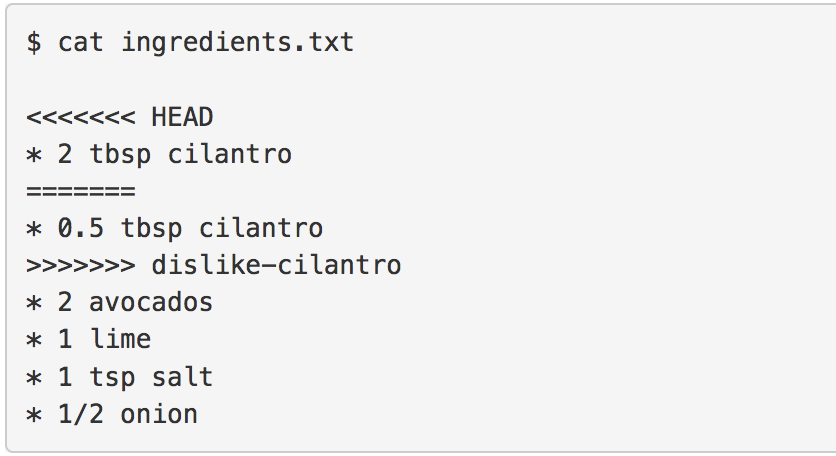
\includegraphics[width=0.7\textwidth]{pics/git_conflict.png}
\end{center}

\begin{itemize}
 \item TALK to the other person(s), who made the conflicting changes, and
       find a common solution
 \item choose the version, you agree on (not necessarily either of yours)
 \item remove the conflict identifiers
 \item add and commit
 \item then proceed with what you where up to
\end{itemize}


\end{frame}

\begin{frame}{Best practice}


\begin{itemize}
 \item AVOID conflicts
 \item branch off for every single feature
 \item merge often
 \item do not merge buggy code anywhere, where it can affect somebody else's
       unrelated work
\end{itemize}


\end{frame}


\begin{frame}{Exercise}

\begin{enumerate}
 \item create local branch tracking \emph{your grgoup's} remote branch
 \item branch off
 \item add you name to the list of main authors in your document
 \item safely move this change to your group's remote branch using the
       strategy given in this document
 \item resolve conflicts along the way
 \vfill
 \item move on collectively adding content to your topic
 \item goal: have all contributions on the remote branch until 17.50/16.50
\end{enumerate}

\end{frame}


\end{document}
